% !TEX encoding = UTF-8
% !TEX TS-program = pdflatex
% !TEX root = ../tesi.tex
% !TEX spellcheck = it-IT

%**************************************************************
\chapter{Milestone}
\label{cap:milestone}
%**************************************************************

%**************************************************************
\section{Milestone S.r.l. nel mercato}

Milestone si pone come software house di spicco nel settore dei videogiochi a livello mondiale. Grazie all'esperienza acquisita nel proprio ambito (racing) riesce a competere con case produttrici molto più grandi e blasonate senza per niente sfigurare.\\

Attualmente l'azienda sviluppa i propri giochi per le seguenti piattaforme: PC, Sony Playstation Vita\textsuperscript{\textregistered}, Sony Playstation 3\textsuperscript{\textregistered}, Sony Playstation 4\textsuperscript{\textregistered}, Microsoft Xbox 360\textsuperscript{\textregistered} e Microsoft Xbox One\textsuperscript{\textregistered}. Quest'ultima piattaforma al momento non ha ancora avuto un titolo Milestone nello scaffale ma, visto l'attuale impegno, un primo titolo per Xbox One\textsuperscript{\textregistered} non tarderà ad arrivare.\\

Come già detto, i prodotti Milestone sono venduti in tutto il mondo. Il solo mercato italiano procura il 12\% del fatturato aziendale. Il resto del ricavato arriva principalmente dall'Europa in cui Milestone ha una lunga tradizione. Di recente acquisizione è il mercato Americano, dove verrà a breve distribuito un nuovo gioco grazie ad un accordo di sub-licensing con Namco Bandai. Anche nel resto del mondo: Giappone, Russia, Australia e Sud Africa i giochi sono distribuiti tramite accordi di sub-licensing\footfullcite{site:accordo-namco-bandai}.\\

La divisione dei ricavati sulle varie piattaforme indica la rapida crescita delle console di ultima generazione, confermando anche per i giochi Milestone la stessa tendenza (Xbox One\textsuperscript{\textregistered} al momento esclusa). Ricopre invece un ruolo marginale il mercato PC, la cui quota è davvero minimale.\\

Milestone vende sia in formato digitale tramite gli store di Sony, Microsoft e Valve (Steam), sia in formato retail con CD e copertina rigida. La produzione delle copie retail e la distribuzione fisica nei negozi è appaltata esternamente.\\

Milestone è una delle poche aziende al mondo che ricopre anche il ruolo di Publisher. Questo ruolo consiste nel dialogo con Sony e Microsoft per accordare la pubblicazione di un videogame sulle loro console. Solitamente, la maggior parte delle software house, si affida ad aziende terze. Ricoprire questo ruolo internamente consente all'azienda di avere un dialogo diretto con i console owner, permettendo una più rapida interazione. Per capire il motivo per il quale un rapido dialogo sia così importante bisogna introdurre le TRC/TCR\footfullcite{site:approfondimento-TRC}. Esse sono delle condizioni tecniche/qualitative che i giochi devono rispettare per essere pubblicati sulle console. Ogni console ha le sue specifiche. I console owner hanno interi team per testare i game secondo le TRC/TCR e quindi l'utilità di questo reparto si spiega da sola\footfullcite{site:approfondimento-game-testing}. Lo scopo delle TRC/TRC è quello di assicurare un alto standard qualitativo del software che viene distribuito sulle console. Inoltre è uno strumento utilizzato dai console owner per poter meglio controllare l'universo attorno le loro console.\\

La curva dei profitti in relazione all'uscita del gioco sul mercato è molto semplice. Nel primo mese a partire dal \gloss{Day One} si concentra la maggior parte del profitto dell'intera vendita del videogame. Al passare del tempo inizia un repentino calo delle vendite e ribasso del prezzo. Nel frattempo inoltre escono titoli concorrenti più nuovi che contribuiscono alla tendenza. Dopo la rapida decrescita si succede una fase molto più lenta che prosegue fino alla morte del prodotto.


%**************************************************************
\section{Pirateria}

Nel contesto della curva di profitto di un gioco si inserisce la lotta contro la pirateria. L'azienda si affida, per la protezione anti-copia, a software diversi in base alla piattaforma target. Per le console tutte le aziende del settore, tra cui Milestone, si affidano ai meccanismi anti-copia offerti dai console owner per le proprie piattaforme. Su PC l'azienda si affida a Solid Shield\footnote{\url{http://www.solidshield.com/}} per le versioni retail e alla protezione build-in offerta da Steam.\\

Il problema della pirateria informatica su PC è sempre stato molto sentito dalle software house, in quanto in Microsoft Windows\footnote{Microsoft Windows è il sistema maggiormente diffuso sul quale vengono giocati i videogiochi su PC e per questo viene preso ad esempio}, essendo un sistema operativo aperto, risulta molto più semplice ovviare alle protezioni digitali anti-pirateria rispetto alle console, sulle quali gira un sistema chiuso in cui non è permesso installare software non pre-approvati dal console owner.\\

Solid Shield funziona in maniera trasparente al codice del gioco, in quanto, una volta prodotto l'eseguibile finale di esso, questo viene passato a loro, i quali costruiscono un guscio esterno di protezione sbloccabile soltanto con un codice valido, solitamente distribuito insieme alla copia del gioco.\\

Su Steam invece la fase di sviluppo passa attraverso un utente aziendale riconosciuto come sviluppatore di quel particolare gioco, il quale lo può avviare anche senza possederlo nella propria libreria, a patto di avere un file nella stessa cartella dell'eseguibile con all'interno il codice identificativo segreto del gioco. L'hacking della protezione Steam passa proprio attraverso questo meccanismo, scoprendo il codice segreto e facendo credere al sistema di essere un utente sviluppatore.\\

Al momento PS3\textsuperscript{\textregistered} e Xbox 360\textsuperscript{\textregistered} sono le uniche console, per cui Milestone sviluppa, che sono state \gloss{hackerate} e compromesse.
PS3\textsuperscript{\textregistered}, ad esempio, è stata violata quando era presente il firmware versione 3.55. La casa è riuscita però a proteggere tutte le console che sono nate con o sono state aggiornate a firmware successivi. Rimangono però attualmente scoperte le console non aggiornate per via ufficiale. Sony ha quindi attuato politiche di \gloss{ban} definitivo dal Playstation Network\textsuperscript{\textregistered} (\gloss{PSN}) delle console hackerate. La comunità pirata ha però nel tempo rilasciato versioni modificate che permettono a coloro che ha come base una console con firmware 3.55 o inferiore di installare nuove versioni aggiornate dello stesso con protezioni anti-ban per permettere comunque l'accesso al PSN\textsuperscript{\textregistered}. Ne è susseguita una danza ciclica in cui Sony rilasciava un nuovo firmware che correggeva il buco di protezione seguito dopo poco da un rilascio di un nuovo firmware che trovava un altro modo per permettere comunque di averne uno aggiornato e la protezione per l'accesso al PSN\textsuperscript{\textregistered}. Inoltre i nuovi giochi richiedono espressamente versioni del firmware molto recenti per proteggersi da copie hackerate del firmware non aggiornate.\\

Da tutto questo ne consegue quindi uno sforzo contro la pirateria da parte di Milestone solo nelle primissime fasi dopo il day one, successivamente tra prezzi scontati, calo delle vendite e azione della pirateria limitata quasi soltanto al PC, dal quale provengono una piccolissima parte dei ricavati, non giustificano lo sforzo economico per continuare la battaglia.

%**************************************************************
\section{Suddivisione della forza lavoro}

Milestone S.r.l. conta ad oggi circa 120 impiegati, di questi circa 90 appartengono ai reparti che si occupano dello sviluppo, ovvero creazione degli asset (modelli 3D, piste, animazione ecc), programmazione e game design. Il resto si occupa del publishing (circa 10 persone), della pianificazione a lungo raggio e management aziendale, del quality assurance (QA), del configuration e data management, delle human resources (HR), della amministrazione e del settore IT.\\

Il team di Human Resources si occupa di gestione del personale. Suo il compito di selezionare e arruolare nuove leve, promuovere o licenziare personale. Essendo personale non tecnicamente specializzato in game development si affida ai team leader per eseguire le valutazioni tecniche dei candidati.\\

Il team di configuration e data management si occupa di gestire l'utilizzo del repository aziendale, tra cui la gestione dei branch. Inoltre si occupano delle build aziendali, la gestione e trasformazione degli asset dai formati nativi dei programmi di sviluppo ai formati compressi e ottimizzati con i quali verranno distribuiti insieme al gioco.\\

L'amministrazione esegue compiti non appartenenti al core business dell'azienda ma comunque indispensabili quali: l'amministrazione del personale, gestione dei locali e molto altro.\\

Il team IT si occupa invece della manutenzione e della gestione del parco macchine PC aziendale. Gestisce tecnicamente i server e tutti i vari servizi (esempio: mail, MantisBT).\\

Ogni reparto ha il proprio leader che sovrintende e gestisce i lavori. Ricorsivamente ogni reparto è suddiviso in team, i quali hanno a loro volta il proprio leader. I leader sono coloro che si occupano della pianificazione. Nel momento in cui la direzione necessita di una pianificazione su un nuovo progetto essa la chiede ai tre leader principali (programmazione, artist e game designer), i quali a loro volta la girano ai sotto leader e, ottenuti i risultati delle varie parti compongono la stima totale.\\

Esiste un'altra organizzazione di leader trasversale ma complementare alla precedente. Ogni reparto ha un team leader per progetto (videogame). Questa organizzazione è detta \dq{matriciale} ed è importantissima poiché i giochi contemporaneamente sviluppati sono sempre almeno 2 e, mentre i team leader normali hanno la visione generale, i team leader per game mantengono l'obiettivo del singolo game evitando di disperdere le energie.\\

Il team di QA ha il compito di scovare e segnalare tutti i \gloss{bug} presenti sui prodotti. Essi tracciano tutti gli errori scovati tramite l'utilizzo del tool open source MantisBT\footnote{\url{https://www.mantisbt.org/}}. MantisBT è un famoso strumento che permette la segnalazione di bug e la gestione completa fino alla risoluzione. Esso è stato personalizzato e adattato alle esigenze specifiche dell'azienda, ottenendo uno strumento semplice ma potente.\\

La procedura prevede che il personale del QA segnali il bug scovato e tutti i dettagli per riconoscerlo e riprodurlo, inoltre ne assegna la risoluzione al team di programmazione più pertinente. A questo punto il team leader che riceve il bug decide a chi farlo risolvere all'interno del proprio team, seguendo la regola di assegnarlo alla persona che si suppone possa sistemarlo nel minor tempo possibile. È prevista la possibilità che il team leader riassegni il bug ad un altro reparto, ma solo se il team di QA abbia sbagliato oppure se la risoluzione avverrà più velocemente dal nuovo team. La direzione tiene traccia di questi \dq{rimbalzi} allo scopo di evitare che il principio di minimo tempo di risoluzione non venga mai meno. Un'ulteriore possibilità è che il team leader, insieme alla direzione, valuti la risoluzione dell'errore di non importanza strategica. A questo punto il bug non verrà mai risolto. Quando il reparto di programmazione segnala un bug come sistemato, il team QA si assicura che il problema sia stato davvero rimosso, altrimenti la procedura ricomincia d'accapo.\\

%\begin{figure} %Non ho lo screenshot di mantis
%	\centering
%	%\includegraphics{screenshot mantis}
%	\caption{Screenshot di MantisBT}
%	\label{fig:screenshot-mantis}
%\end{figure}

Il reparto di sviluppo si divide in 3 reparti: programmazione, artist e game design. Il reparto di artist è quello che si occupa della creazione degli asset per i giochi. I game designer sono coloro che ideano i giochi e decidono come saranno. Essi descrivono dettagliatamente tutti i contenuti, i flussi e le feature che vorrebbero avere in un gioco. Dopodiché i team di programmazione, gli artist e la direzione stimano il tempo necessario e nel caso tagliano qualche contenuto.\\

Il reparto di programmazione si divide nei seguenti team: UI, Online, programmazione 3D, gameplay e R\&D (ricerca e sviluppo).\\

Il team UI scrive e mantiene le pagine di interfaccia utente. Inoltre si occupa dalla gestione della grande macchina a stati finiti che rappresenta il gioco ed il passaggio e la consistenza dei dati in essa (esempio: i dati prestazionali di una moto). Gestisce i salvataggi e trasforma l'input utente in azioni in base al contesto nel quale sono stati premuti. Ad esempio la pressione del tasto X su tutte le Playstation\textsuperscript{\textregistered} seleziona l'azione di l'azione corrente quando un menu è visualizzato, mentre scala una marcia durante lo stato di gara.\\

Il team Online, come suggerisce il nome, gestisce la componente multiplayer online di ogni videogame. Si occupa dal creare e configurare le partite (match making) alla comunicazione di rete durante le gare, fino alla gestione delle \gloss{leaderboard}. La comunicazione online di basso livello si basa sul \gloss{middleware} \gloss{Raknet}\footnote{\url{http://www.jenkinssoftware.com/}}.\\

Il team di gameplay gestisce le meccaniche di gioco in race. Si occupa della simulazione fisica della gara e della gestione dell'AI (Artificial Intelligence) che controlla gli avversari del giocatore.\\

Il reparto di ricerca e sviluppo si occupa dello sviluppo dell'engine grafico, ricercando sempre nuovi soluzioni e tecniche per mantenerlo all'avanguardia nel panorama mondiale. Tutti i giochi si basano sull'engine grafico, denominato GEM. Lo sviluppo di GEM avviene parallelamente allo sviluppo dei giochi, semplicemente quando parte la programmazione di un nuovo gioco viene usata l'ultima release stabile. Questo team si occupa inoltre di tutti gli strumenti a supporto dello sviluppo grafico. Sua responsabilità è lo sviluppo e la manutenzione degli editor di gioco, quali ad esempio il GEM Editor, giunto alla release 2.\\

L'organizzazione dei task per ciascun impiegato è gestita tramite il tool \gloss{Microsoft Project}\footnote{\url{http://office.microsoft.com/en-001/project/}}. Come già spiegato la cura dei task è gestita gerarchicamente dai team leader che assegnano al proprio team.\\

%\begin{figure} %Non ho lo screenshot
%	\centering
%	%\includegraphics{screenshot microsoft project}
%	\caption{Screenshot di Microsoft Project}
%	\label{fig:screenshot-microsoft-project}
%\end{figure}

Il team dove lo stagista è stato inserito è il team 3D, il quale, ad alto livello, utilizza l'engine grafico per disegnare le scene del gioco. Verrà maggiormente approfondito il ruolo del team successivamente alla spiegazione delle fasi di sviluppo di un videogame in Milestone S.r.l.\footnote{Si veda la sezione \ref{sec:ruolo-3D-programmer-workflow}.}

\section{Game workflow}

Lo sviluppo di tutti i giochi in Milestone S.r.l. segue sempre le seguenti fasi:

\begin{enumerate}
	\item Tutto parte da un \textbf{Macro Design} del gioco. Se il gioco è completamente nuovo, oppure se si basa su un altro già completato evolvendolo, si procede a identificare i punti chiave e le feature innovative che si vuol inserire. Con queste in mano si effettua, con le procedure prima descritte, ad una stima di tempo e fattibilità del gioco.
	\item Approvato il progetto si procede alla creazione di un \textbf{Concept Design} e contemporaneamente alla \textbf{pre-production}. Il concept design è un approfondimento, di dettaglio, di come sarà il gioco, sarà la base ufficiale sulla quale verrà tecnicamente progettato e sviluppato. Una versione più ridotta viene inviata a Sony e Microsoft, in modo tale da ottenere il loro permesso per poter pubblicare quel gioco sulle loro console. la pre produzione è invece l'inizio della progettazione della struttura degli asset e l'inizio della loro creazione. Si vuole informare il lettore che la quantità di asset necessaria per lo sviluppo di un titolo \gloss{AAA} è davvero enorme. L'azienda procederà quindi ad appaltare esternamente lo sviluppo di parte di questi.
	\item Terminata la fase di design si procede alla creazione di un \textbf{prototipo} nel quale saranno presenti le feature più innovative e complesse del gioco. È da questo momento che la programmazione ha inizio. Le feature inserite sono solitamente stabili e testabili. Il prototipo è un ibrido tra incrementale ed usa e getta, ad esclusivo utilizzo interno. L'utilità di questo prototipo è saggiare se le nuove feature, le più complesse, sono fattibili nei tempi pianificati e soprattutto verificare la realizzabilità. Procedere subito a testarle permette di poter correggere subito il tiro in caso di problemi, evitando il fallimento del progetto, inevitabile se problemi del genere fossero scoperti troppo tardi.
	\item Questa fase è un misto tra una classica \textbf{\gloss{First Playable}} ed una \textbf{\gloss{Vertical Slice}}. L'azienda ha deciso di unificare queste due fasi che solitamente tendono ad essere separate. La motivazione è prettamente strategica, in quanto la realizzazione del prototipo ha provveduto già ad evidenziare le maggiori difficoltà e dato l'alto numero di giochi sviluppati contemporaneamente, una compressione a questo punto risulta del tutto accettabile. L'esperienza del team sui giochi di corsa, aiuta inoltre a poter gestire l'unione delle due fasi. Da questa fase esce quindi un prototipo incrementale ad uso pubblico. Esso è molto più simile ad una first playable poiché gli asset, vista la loro vastità, tendono ad arrivare in versione finale molto tardi. Solitamente viene mostrato ai giornalisti di tutto il mondo. Si vuol evidenziare come a partire da questa fase la velocità di sviluppo cresce repentinamente, così come l'impegno complessivo dedicato al gioco in termini di risorse investite.
	\item A questo punto si arriva alla cosiddetta versione \textbf{Alpha} del gioco in cui tutti gli asset presenti richiedono memoria e prestazioni in gioco come i definitivi. Per evitare equivoci tutto ciò che non è definitivo viene marcato come tale. In questo modo sia i giornalisti che i developer possono riconoscere e ricordare ciò che deve essere completato. Le feature sono state tutte inserite, magari non complete e/o completamente stabili ma presenti. È possibile così valutare le prestazione e le performance di gioco e, nel caso venissero riscontrati problemi c'è ancora tempo per risolverli.
	\item La \textbf{Beta} presenta tutti gli asset nella loro versione finale. Tutte le feature iniziano a diventare stabili ed il reparto di QA svolge un ruolo molto importante in questa fase, alla ricerca di tutti i bug.
	\item Quando la direzione ritiene il gioco abbastanza stabile, si procede alla \textbf{Submission} tramite il reparto di publishing, il quale inoltra una copia del gioco ai console owner, Microsoft e Sony, allo scopo di ottenere l'approvazione per la pubblicazione definitiva del gioco. Per ottenerla, i giochi sono testati, secondo le TRC/TCR per ciascuna console. Questa fase è davvero delicata in quanto ogni submission richiede circa due settimane ed in caso di fallimento, bisogna rifare la procedura fino ad ottenere l'approvazione. Fallire le submission comporta innanzitutto una preziosa perdita di tempo e secondariamente, una perdita economica. In quanto, per ciascun gioco, per ciascuna piattaforma, le submission dalla terza in poi iniziano a costare davvero salate e conseguentemente a pesare sul budget. È quindi priorità dell'azienda superare le submission al primo tentativo.
	\item \textbf{Gold} è il nome della versione finale, completamente stabile senza bug gravi, pronta per essere distribuita worldwide.
\end{enumerate}

\section{Ruolo dei 3D programmer nel workflow}
\label{sec:ruolo-3D-programmer-workflow}

Durante la seconda fase i 3D programmer progettano insieme agli artisti la struttura sulla quale verranno creati gli asset. Per essere concreti, ad esempio, dell'asset di una moto, decidono in quanti e quali modelli sarà suddivisa la \gloss{mesh}. Come saranno le \gloss{texture} e molto altro. Fissata la struttura potranno poi gli artisti (interni ed esterni), creare tutti gli asset necessari.\\

Durante tutto lo sviluppo essi scrivono e/o aggiornano il codice necessario alla gestione in memoria degli asset. Questo è un compito molto delicato in quanto deve tener conto di diverse necessità ed effettuare una sintesi scrupolosa. La necessità primaria è la velocità di caricamento, in un mondo ideale si vorrebbe avere tutti gli asset caricati in memoria centrale pronti per essere usati (todo mettere riferimento al capitolo 3 in cui si introduce una strategia per svolgere questo compito). Nella realtà invece il programmatore si scontra con i diversi limiti hardware delle varie piattaforme target, è quindi costretto a implementare logiche intelligenti e molto efficienti.\\

Caricare gli asset in memoria significa inoltre riassemblarli. Per non sprecare spazio, ogni componente degli asset che serve più di una volta, viene memorizzata una volta sola nei dati grezzi. Questo significa che per ricomporre un oggetto 3D, bisogna recuperare tutti i sotto componenti e ricomporre la struttura ad albero originale. Esiste ovviamente un database, nei giochi Milestone scritto in linguaggio \gloss{XML}, in cui è scritto come ricomporre le strutture originali degli asset.\\

\begin{figure}[!h]
	\centering
	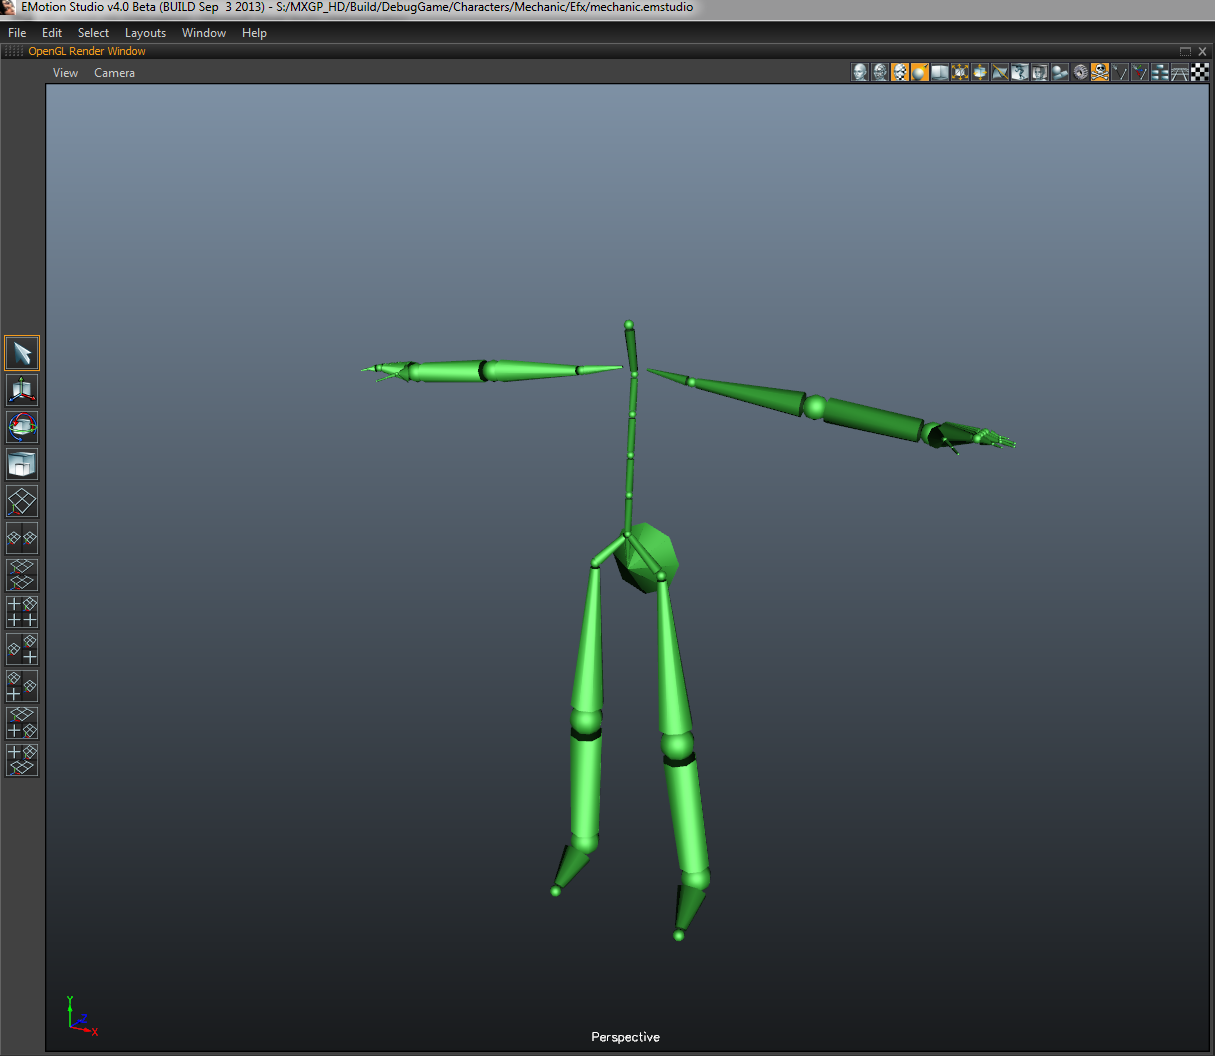
\includegraphics[width=1.0\columnwidth]{game/emotionStudioSkeleton.png}
	\caption{Screenshot di EMotion Studio durante la visualizzazione dello skeleton di animazione di un meccanico in T-pose}
	\label{fig:screenshot-emotion-studio-1}
\end{figure}

\begin{figure}[!h]
	\centering
	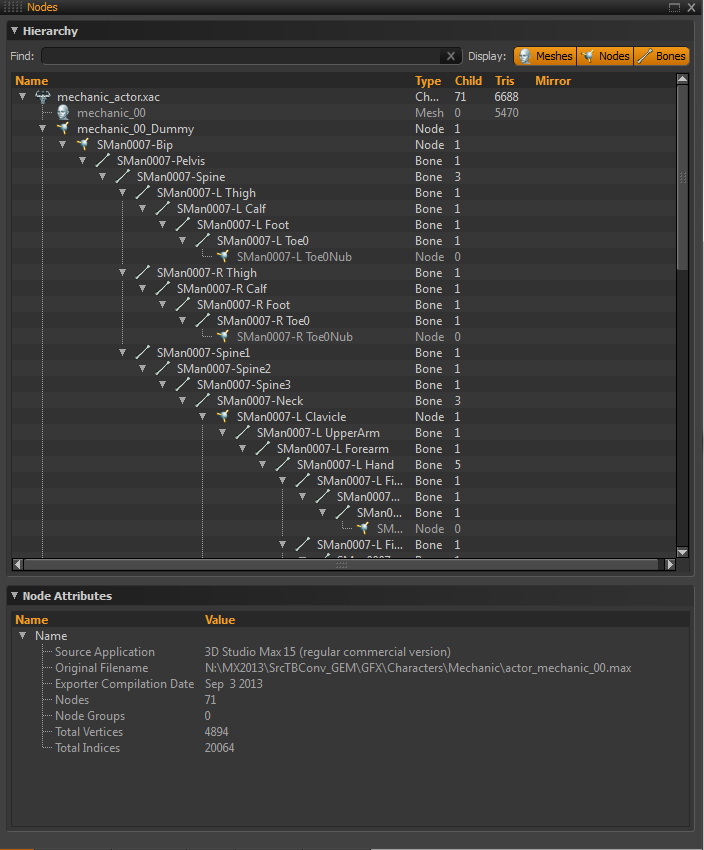
\includegraphics[width=1.0\columnwidth]{game/emotionStudioHierarchy.png}
	\caption{Screenshot di EMotion Studio durante la visualizzazione della gerarchia dei bone di animazione dello skeleton di un meccanico}
	\label{fig:screenshot-emotion-studio-2}
\end{figure}

Altra responsabilità è l'utilizzo dell'engine GEM per disegnare le scene 3D richieste dal design del gioco. Il mondo di gioco viene gestito a \dq{World}, questo significa che tutti gli oggetti 3D sono contenuti all'interno di questo mondo. Compito del team è scrivere un'implementazione efficiente del World per disegnare tutti gli oggetti presenti.\\

I World si dividono in ambienti di gara e non. Negli ambienti non di gara il team gestisce anche le cosiddette \textbf{cut-scene}, esse sono le scene in cui il giocatore è spettatore passivo della scena 3D. Un esempio è la sequenza animata che simula la cerimonia del podio alla fine di una gara. In Milestone S.r.l. esistono due sistemi di gestione delle cut-scene. Il primo, in ordine temporale di adozione, prevede la descrizione della scena in linguaggio XML (MotoGP 14), mentre il secondo utilizza degli script \gloss{LUA}\footnote{Per maggiori approfondimenti \fullcite{inbook:game-coding-complete} e \fullcite{site:lua-paper}} (MXGP).\\

Ultimo ma non meno importante compito, è la gestione degli ambienti di gara. In essi il team gestisce il collegamento degli oggetti 3D con la simulazione fisica, la quale evolve i parametri degli oggetti di gioco. Tramite questi parametri si richiede l'esecuzione dell'animazione, la quale aggiorna i parametri visibili degli oggetti 3D, ad esempio la posizione.\\

Per eseguire le animazioni il team utilizza il middleware EMotion FX 4\footnote{\url{http://www.mysticgd.com/website/index.php?id=17}} , il quale dato il blend tree sviluppato dagli artisti, esegue in real time le animazioni sugli oggetti 3D. Gli artisti, in Milestone, sviluppano i blend tree tramite il tool EMotion Studio fornito dalla stessa casa.

\section{Configuration e data Management}

Il software di versionamento utilizzato in Milestone è \gloss{Perforce}\footnote{Per il lettore appassionato è disponibile una semplice ma efficacie introduzione a Perforce\textsuperscript{\textregistered} al seguente link: \url{http://www.perforce.com/perforce/doc.current/manuals/intro/intro.pdf}}, che recentemente ha rimpiazzato \gloss{Alienbrain}. Un punto di forza che distingue Perforce\textsuperscript{\textregistered} dagli altri software di versionamento sono gli Stream. Questi sono dei branch intelligenti, in altre parole, al posto di effettuare una copia vera e propria per creare un branch, come fanno ad esempio Git\textsuperscript{\textregistered} ed SVN\textsuperscript{\textregistered}, qui sono gestiti interamente in termini di \gloss{delta} rispetto al branch master. Altra particolarità e la modalità di commit su shelve (scaffale). Tale modalità permette di eseguire il commit (check-in in Perforce\textsuperscript{\textregistered}) su uno spazio personale. Questo significa che un altro programmatore quando eseguirà la get (pull in Git\textsuperscript{\textregistered}, update in SVN\textsuperscript{\textregistered}) non otterrà la versione in shelve. Dovrà manualmente richiederla per poterla avere. Questa modalità risulta molto utile ad esempio per eseguire il commit di alcune modifiche che non sono ancora state testate, oppure sono una soluzione alternativa in attesa di approvazione.

\section{Asset}
\label{sec:asset}

Come già accennato, gli asset subiscono una serie di trasformazioni prima di arrivare nella forma che viene distribuita insieme al gioco. Essi possono essere trovati in uno dei seguenti stati:
\begin{enumerate}
	\item \textbf{rough}: i dati sono nella forma originale fornita dall'artista. Tipicamente sono nel formato nativo del programma con il quale sono stati sviluppati.
	\item \textbf{middle}: i dati sono parzialmente ottimizzati, tramite compressione e \gloss{serializzazione} (se ad esempio il formato originale era XML).
	\item \textbf{final (mixed)}: i dati sono stati unificati in pochi file chiamati \dq{mixed}. Da migliaia di file si passa ad una manciata di grossi file con estensione \dq{.mix}.
\end{enumerate}

\begin{figure}[t]
	\centering
	\hspace*{-0.05\columnwidth}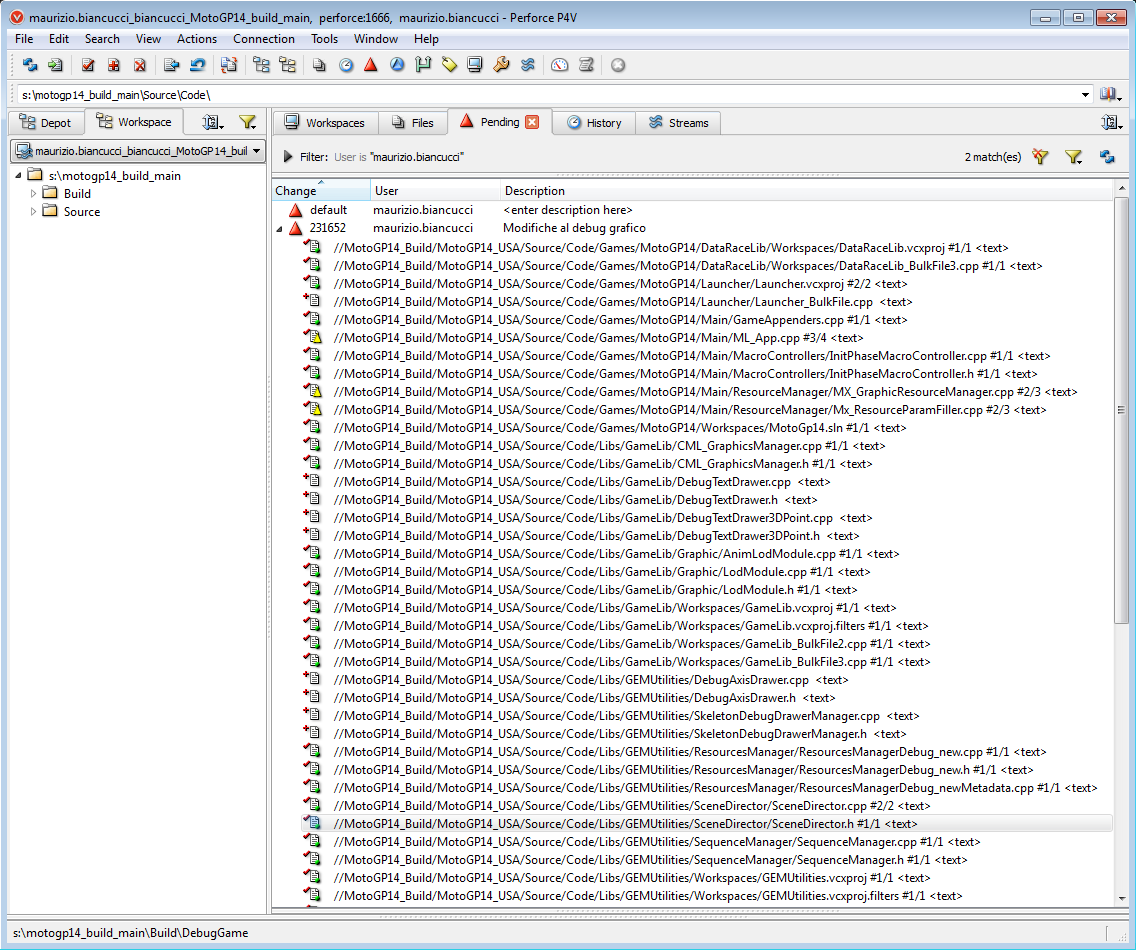
\includegraphics[width=1.1\columnwidth]{game/perforce.png}
	\caption{Screenshot di Perforce}
	\label{fig:perforce}
\end{figure}

La trasformazione degli asset nel formato finale ha un duplice scopo. Essendoci pochi ma grandi file le performance del gioco in fase di caricamento aumentano notevolmente\footnote{Si ricorda al lettore la lentezza degli hard disk tradizionali, o anche peggio dei CD, nel leggere tanti piccoli file, anche se fisicamente contigui}. Inoltre, avendo convertito gli asset in un formato proprietario (il \dq{.mix}), si corre meno il rischio che gli asset possano essere \dq{rubati} e riutilizzati senza il permesso dell'azienda.\\

In Milestone S.r.l. è presente un \gloss{sistema di integrazione continua} che ogni notte procede a eseguire le \gloss{build} di tutti gli asset aggiornati. Viene eseguita una build per ogni stato disponibile. Ogni build termina con una mail collettiva (agli interessati) con gli esiti. Nel caso la build fosse stata rotta, viene mandata una mail a tutti coloro che hanno contribuito a modificare l'asset fallito. La procedura di build è stata settata per utilizzare tutti i PC dell'azienda contemporaneamente. Questo è molto importante poiché, vista l'enorme quantità di asset da convertire, di molteplici giochi, è l'unico modo per poter riuscire a finire tutto entro la mattina successiva. La pecca di questo sistema è che, per poter visionare e testare le modifiche agli asset nei formati n\textdegree 2 e 3, bisogna per forza aspettare il giorno lavorativo successivo.

\section{Code build}

Tutti i giochi Milestone sono sviluppati contemporaneamente per molte piattaforme\footnote{link a dove si dice quali sono le piattaforme}. Questo comporta l'utilizzo contemporaneamente di molti compilatori. Ogni piattaforma ha il suo compilatore, ad esempio sia Sony, sia Microsoft hanno sviluppato un compilatore proprietario per le proprie console. Questo comporta una sforzo aggiuntivo da parte di tutti i programmatori, i quali si devono assicurare che il codice scritto compili e funzioni correttamente su ciascuna piattaforma prima di eseguire la commit.\\

Sono state definiti diversi target di compilazione, i quali variano per quantità di ottimizzazione e capacità di interazione con i diversi stati degli asset:
\begin{enumerate}
	\item \textbf{debug}: build completamente non ottimizzata a totale scopo di debug;
	\item \textbf{release}: non standard, è parzialmente ottimizzata ma contiene ancora i simboli per il debug;
	\item \textbf{official}: build completamente ottimizzata. Si invita il lettore a prestare attenzione alla differenza con lo stato \dq{final} degli asset.
\end{enumerate}

I target debug e release hanno la capacità di leggere gli asset in tutti gli stati possibili. La official invece, può utilizzare solo le versioni final. Tipicamente le combinazioni utilizzate sono le seguenti:
\begin{enumerate}
	\item \textbf{debug/release target + rough asset}: per debug. Soffre della lentezza di caricamento determinata dagli asset divisi in tantissimi piccoli file. Date le limitate capacita di PS3\textsuperscript{\textregistered}, 256 MB di RAM, capita che verso le fasi finali di sviluppo non si riesca ad avviare questa combinazione.
	\item \textbf{official target + final asset}: è la versione per l'utente finale e solitamente usata dal QA.
	\item \textbf{debug/release target + final asset}: molto più veloce a caricarsi, è utilissima per testare una modifica sul codice che non coinvolge gli asset.
\end{enumerate}

Come il lettore può aver intuito, il codice di gioco si compone di moltissime librerie, le quali contengono complessivamente migliaia di file. Allo scopo di ridurre significativamente i tempi di compilazione, si è adottata la tecnica di compilazione \textbf{bulk}. Essa consiste semplicemente nel creare un unico file per libreria, nel quale si includono tutti i cpp. Altra tecnica usata è l'utilizzo delle \textbf{forward declaration} nei file header. Diminuendo gli include e sostituendoli con le dichiarazioni incomplete, si riesce a tenere sotto controllo l'esplosione dei tempi di compilazione.\\

Al momento, tutti i giochi Milestone per PC si basano sul compilatore di Visual Studio 2010, il quale supporta in maniera sperimentale il C++ 11. È scelta aziendale quella di rimandare l'utilizzo del C++ 11 a quando l'implementazione diventerà quasi identica fra i compilatori attualmente usati. Si ipotizza di iniziare ad usarlo quando si passera all'ultima versione del compilatore di Microsoft.\\

Anche per il codice di gioco, è in atto un sistema di integrazione continua, il quale usa le stesse procedure di quello utilizzato per gli asset.\footnote{Per ulteriori dettagli si inviata il lettore a consultare la sezione \ref{sec:asset}}.

\section{Metadati}

I giochi Milestone utilizzano il sistema dei metadati. Lo scopo è di ottenere delle funzionalità simili alla riflessione anche in C++. Queste funzionalità spaziano dal real-time editing delle variabili, update da e verso XML e/o binari. Questa tecnica permette uno scambio di dati disaccoppiando le due classi a discapito del controllo degli accessi. È infatti possibile esporre come metadati anche membri di classe privati.\\

Tutti i metadati presenti sono esposti via rete, solo nei target debug e release, nel \textbf{Beholder}. Questo è un client che permette la visualizzazione e l'editing in tempo reale dei metadati. Un efficacie esempio di utilizzo è l'esposizione nel beholder di dati XML, seguito dal tuning in real time di codesti dati, e il salvataggio automatico dei nuovi valori se soddisfatti del risultato.\\

Un altro esempio di utilizzo del Beholder, molto usato dal team 3D, è l'esposizione di funzioni attivabili direttamente dall'interfaccia grafica di quest'ultimo. Le più usate sono quelle per disegnare geometrie di debug, quali ad esempio gli assi di origine degli spazi di riferimento degli oggetti presenti nelle scene 3D.\\

L'utilizzo dei metadati all'interno del codice avviene tramite un set di macro definite in GEM. Un facile esempio di utilizzo è il seguente.

\begin{lstlisting}[style=maurizio-code, caption=Dog.h, label={code:metadata-example-h}]
class Dog
{
public:
	ENABLE_METADATA;

	// methods
	void Walk();
	void Jump();

	// events
	TypedEvent<> OnFall;
	TypedEvent< GString > OnDie;

private:
	int m_age;
	float m_weight;
};
\end{lstlisting}

Di seguito è presente il codice per eseguire l'esposizione di tutta la classe nei metadati.

\begin{lstlisting}[style=maurizio-code, caption=Dog.cpp, label={code:metadata-example-cpp}]
META_BEGIN_CLASS( Dog )

META_BEGIN_PROPERTIES
META_NAMED_PROPERTY("Age", m_age),
META_NAMED_PROPERTY("Weight", m_weight)
META_END_PROPERTIES

META_BEGIN_ACTIONS
META_ACTION( Walk ),
META_ACTION( Jump ),
META_END_ACTIONS

META_BEGIN_EVENTS
META_EVENT( OnFall ),
META_EVENT( OnDie ),
META_END_EVENTS

META_END_CLASS
\end{lstlisting}

\section{Norme di codifica}

Allo scopo di uniformare il codice prodotto ed aumentare la comprensibilità, l'azienda ha deciso di adottare la notazione ungherese, alla quale sono state applicate delle piccole personalizzazioni.\\

Tutto il codice è scritto in lingua inglese, compresi i commenti e le annotazioni. Di seguito viene presentato un piccolo riassunto delle regole della notazione adottata in Milestone S.r.l.\\

\begin{itemize}
	\item \textbf{prefissi:}
	\begin{itemize}
		\item \textbf{m}: usato per le variabili membro (esempio: \texttt{m\_keyName});
		
		\item \textbf{s}: usato per le variabili membro statiche (esempio: \texttt{s\_numInstance});
		
		\item \textbf{p}: usato per le variabili puntatore (esempio: \texttt{m\_pkeyNameList});
		\item \textbf{sigla del tipo}: usato per indicare il tipo delle variabili di tipi primitivi (esempio: \texttt{uiGroupIndex});
		
		\item \textbf{i}: usato per le variabili input alla funzione che sono usate come dati di input(esempio: \texttt{i\_resource});
		
		\item \textbf{o}: usato per le variabili input alla funzione che sono usate come output (esempio: \texttt{o\_foundKeys}).
	\end{itemize}
	\item \textbf{capitalizzazione:}
	\begin{itemize}
		\item \textbf{variabili e parametri}: iniziano sempre in minuscolo e usano una lettera minuscola per ogni parola (esempio: \texttt{m\_parentWidget}, \texttt{returnValue});
		\item \textbf{macro ed enum}: completamente in maiuscolo con le diverse parole separate dal carattere \sq{\_} (esempio: \texttt{UPDATE\_CODE});
		\item \textbf{classi, funzioni e metodi}: iniziano sempre in maiuscolo e ogni parola diversa parte in maiuscolo (esempio: \texttt{CObject3d});
	\end{itemize}
\end{itemize}

\section{Assert e Log}

GEM fornisce anche un utilissimo meccanismo di logging. Esso viene messo a disposizione tramite la classe statica LogManager. Il programmatore deve semplicemente settare il contesto, la severità e il messaggio. La vera importanza del sistema di logging unificato deriva dal fatto che, in questo modo, ciascun programmatore può settare i contesti per i quali vuole visualizzare i log.\\

Altra funzionalità offerta da GEM sono un set di assert personalizzato. Questi assert sono scartati dalla compilazione nei target release e official. Un corretto utilizzo degli assert è quello di inserirne uno per ciascuna precondizione. In altre parole, molto spesso, le funzioni si basano su delle condizioni che assumono vere al momento dell'invocazione, condizioni che sono alla base della correttezza dell'algoritmo. Se invece di spiegarle con commenti testuali, si utilizza una assert, esse sono sempre verificate a run-time e aiutano efficacemente a scovare bug molto difficili da trovare con altri mezzi.